\documentclass{beamer}

\usepackage{graphicx}
\usepackage{listings}

\lstset{
  columns=fixed,
  frame=none,
  backgroundcolor=\color[RGB]{245,245,244},
  keywordstyle=\color[RGB]{40,40,255},
  numberstyle=\footnotesize\color{darkgray},
  commentstyle=\it\color[RGB]{0,96,96},
  stringstyle=\rmfamily\slshape\color[RGB]{128,0,0},
  showstringspaces=false,
  morekeywords={terra, if, else, end, int, then, return, struct, float, local, quote, function}
}

\usetheme{AnnArbor}
\usecolortheme{beaver}

\begin{document}
\title{Terra: A Multi-Stage Language for High-Performance Computing}
\author{Zachary DeVito\inst{1} James Hegarty\inst{1} Alex Aiken\inst{1} Pat Hanrahan\inst{1} Jan Vitek\inst{2}}
\institute{\inst{1} Stanford University \inst{2} Purdue University}

\maketitle

\begin{frame}
	\frametitle{Goals}
  \begin{itemize}
  \item Performance matters!\pause
  \item Low-level languages(e.g. C) are good: we need to make best use of features of the target architecture(e.g. vector instructions).\pause
  \item Programming is difficult!\pause
  \item Solution: use high-level languages to generate low-level languages code(e.g. FFTW: OCaml $\rightarrow$ C).
  \end{itemize}
\end{frame}

\begin{frame}
	\frametitle{New Problems}
  \begin{itemize}
  \item In this case, we get three components.\pause
  \item Optimizer: generate plan to guide how to generate code.\pause
  \item Compiler: generate taget code based on the plan.\pause
  \item Runtime: support the generated code and provide feedback to the optimizer.\pause
  \item Problem1: How can we get the runtime statistics in the compiler and generate high-performance code dynamically?\pause
  \item Problem2: How can we re-use legacy libraries?
  \end{itemize}
\end{frame}

\begin{frame}
  \frametitle{Two-Language Design}
  \begin{itemize}
  \item Lua: high-level, dynamically typed, automatic mm, first class functions.\pause
  \item Terra(new!): statically typed, manumal mm.\pause
  \item Use Lua to manipulate Terra code.\pause
  \item Shared lexical scoping, which is hygienic.\pause
  \item Terra code runs independently, to avoid including high-level features.\pause
  \item Lua's stack-based C API makes it easy to interface with legacy code.
  \end{itemize}
\end{frame}

\begin{frame}
	\frametitle{Two-Language Design}
  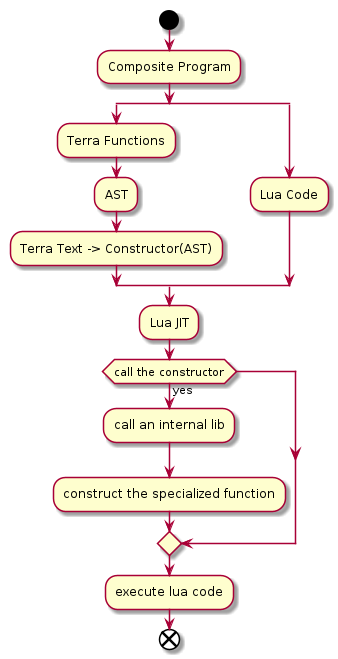
\includegraphics[scale=0.3]{terra.png}
\end{frame}

\begin{frame}[fragile]
	\frametitle{Some Code Examples}
  \begin{lstlisting}
    terra min(a: int, b: int): int
      if a < b then return a
      else return b end
    end
    struct GreyScaleImage {
      data: &float
      N: int
    }
  \end{lstlisting}
\end{frame}

\begin{frame}
	\frametitle{Features}
  \begin{itemize}
  \item Terra entities are all first-class Lua values.\pause
  \item Terra functions will be executed in LLVM JIT.\pause
  \item You can dump Terra functions to an object file(i.e. something.o in Linux) if you like.\pause
  \item Quotation: using brackets($[]$) for escaping and backtick(expressions)/quote keyword(statements) for creating quotation.
  \end{itemize}
\end{frame}

\begin{frame}[fragile]
  \frametitle{Quotation Example}
  \begin{lstlisting}
    local a = 5
    terra sin5()
      return [ math.sin(a) ]
      end
    function addtwo(a,b)
      return `a + b
    end
    local printtwice = quote
      C.printf("hello\n")
      C.printf("hello\n")
    end
  \end{lstlisting}
\end{frame}

\begin{frame}
	\frametitle{It Just Works!}
  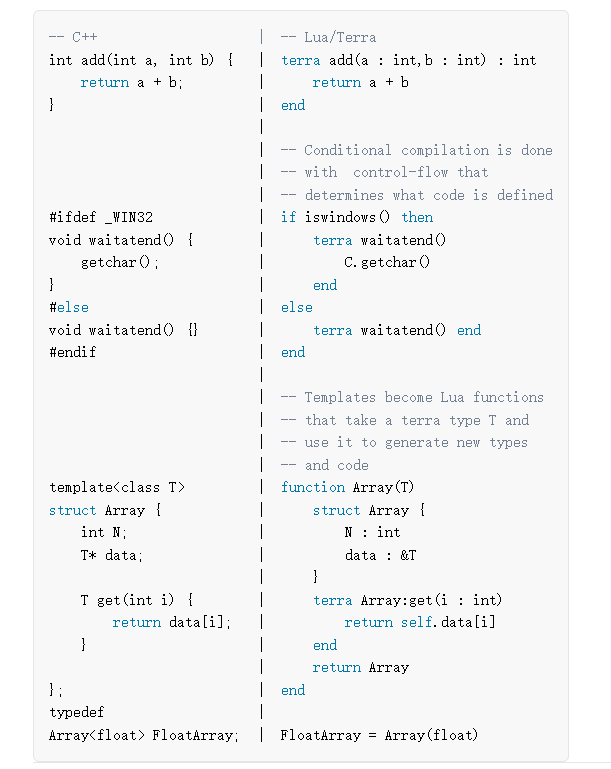
\includegraphics[scale=0.45]{terra2.png}
\end{frame}

\begin{frame}
	\frametitle{It Just Works!}
  \begin{itemize}
  \item Now we can generate code dynamically.\pause
  \item e.g. block the loop nests to make the memory access more friendly to the cache.
  \end{itemize}
\end{frame}

\begin{frame}
	\frametitle{The Formal Calculus: Terra Core}
  % TODO:
\end{frame}

\begin{frame}
	\frametitle{Summary}
  \begin{itemize}
  \item Two-Languages design: Lua + Terra.\pause
  \item Shared lexical scoping.\pause
  \item Seperate Evaluationn: Lua(LuaJIT), Terra(LLVM JIT).\pause
  \item Type Reflection.
  \end{itemize}
\end{frame}

\begin{frame}
	\frametitle{Advantages}
  \begin{itemize}
  \item No need to write C, but the performance is still good.\pause
  \item Generating code dynamically allows us to use runtime information from LuaJIT.\pause
  \item Easy to re-use C/C++ libraries in Lua.\pause
  \end{itemize}
\end{frame}

\begin{frame}
	\frametitle{Shortages}
  \begin{itemize}
  \item Lua is not statically typed.\pause
  \item LLVM + Lua is compromise, because we don't want to re-implement the whole LuaJIT!
  \end{itemize}
\end{frame}

\end{document}

